%%This is a very basic article template.
%%There is just one section and two subsections.
\documentclass[a4paper, 11pt]{article}
\usepackage[pdftex]{graphicx}
\usepackage{parskip}
\usepackage{hyperref}
\usepackage{colortbl}
\usepackage{amsmath}
\usepackage{amsfonts}
\usepackage{enumitem}
\usepackage[left=2cm, right=2cm, top=2cm]{geometry}
\usepackage{float}
\usepackage{afterpage}


\newcommand\blankpage{
    \null
    % \thispagestyle
    \newpage
    }

\newcommand{\points}[1]{(\textbf{#1 marks}) }
\newcommand{\vecthree}[3]{\begin{pmatrix} #1 \\ #2 \\ #3 \end{pmatrix}}
\newcommand{\vecfour}[4]{\begin{pmatrix} #1 \\ #2 \\ #3 \\ #4\end{pmatrix}}
\newcommand{\mat}[1]{\boldsymbol { \mathsf{#1}} }

\begin{document}

\setlength{\parskip}{10pt}
\setlength{\parindent}{0pt}
\DeclareGraphicsExtensions{.pdf,.png,.gif,.jpg}
\begin{center}
	\large
	
\includegraphics[width=3cm, height=3cm]{habib-Logo.jpeg}\\
	\section*{Group project}
	\textbf{Course:} Introduction to Probability and Random Variables -- Spring 2020\\
	\textbf{Instructors:} Dr. Musabbir Abdul Majeed, Dr. Aamir Hasan, Dr. Abdul Samad\\
	\textbf{Date: March 30, 2020}\\
	\textbf{Learning domain level:} COG-4. \textbf{CLOs tested}: 1-5\\
	% \noindent\makebox[\linewidth]{\rule{16cm}{0.4pt}}\\
	% \textbf{ID (just the digits): \underline{\hspace{3cm}}}\\
	% \textbf{\textbf{Circle your section:\hspace{1cm}\Large L1 \hspace{1cm} L2}}
	\section*{Instructions}
	\begin{itemize}
		\item The group project will contribute 15\% towards your final grade. The weightage of Midterm 1 is reduced from 15\% to 10\%   
		\item The project can be done in a group of 2 or 3. If you can't find a group partner, you will have to complete the project on your own
		\item The project must be submitted via LMS and the deadline to submit the project is \underline{18:30 hours on Friday of week 14} 
		\item After the submission, the instructor will arrange a brief Q\&A session to assess your understanding of the project and any question he may have
		\item Your write-up must be no more than 2 pages. Please provide a link to your Github repository and also make sure that it is accessible to the instructors.
		\item There is a zero tolerance policy towards plagiarism and/or collusion. If a student(s) is found to have plagiarised and/or colluded, they will be reported to the academic code of conduct committee which would affect your academic standing in the university. If you are unsure whether you are plagiarising, please ask. Please clearly cite your sources
		\item Following late submission policy will apply:
		\begin{center}
	    	\begin{tabular}{ | l | l |}
			    \hline
			    \# hours past the deadline & Percentage penalty on assignment  \\ \hline
			    $<$ 1 hour & 5\% \\ \hline
			    1-2 hours & 15\% \\ \hline
			    2-3 hours & 30\% \\ \hline
			    3-4 hours & 45\% \\ \hline
			    $>$4  hours & 0\% (not accepted) \\ \hline
		    \end{tabular}
		\end{center}
	\end{itemize}
\end{center}

\newpage

\section{Purpose} 
The purpose of this project is to familiarize students with the modeling of random variables through simulations in any appropriate software environment (Like MATLAB, LabVIEW etc.). This exercise will allow students to generate random variables and their functions so that modeling of real-world situation can be modeled and simulated.  This students will also see how the concepts used in theory classes can be applied in practical situations. As a result of completing this project, you will be able to generate and model some simple random variables probability mass and density functions using built-in random models (like uniform probability) in MATLAB or LabVIEW.   

% you are asked to generate and demonstrate (visually) a model of mobility based on random walks.  
\textbf{Random walk} -- a random walk is a mathematical object, known as a stochastic or random process, that describes a path that consists of a succession of random steps on some mathematical space such as the integers. Mathematical modelling of the movement of animals, micro-organisms and cells is of great relevance in the fields of biology, ecology and medicine. Movement models can take many different forms, but the most widely used are based on the extensions of simple random walk processes.

Figure~\ref{fig:1} shows a simple one-dimensional random walk model where the object (shown in black circle) either moves right or left with probability $p$ and $(1-p)$ respectively. A slightly more complicated random walk model may have the probability that the object stays in place. 

\begin{figure}[h]
\begin{center}
	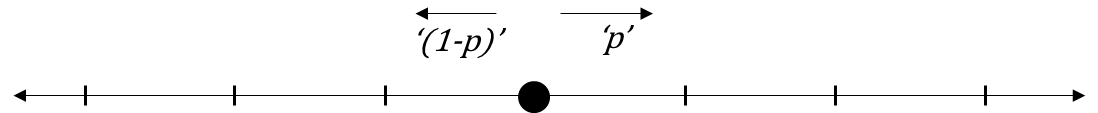
\includegraphics[scale=0.9]{simpleRandomWalk.jpg}
\end{center}	
\caption{one dimensional random walk model}
\label{fig:1}
\end{figure}

After, taking $n$ steps, the position of the node, or expected distance from the start or the expected distance from some destination can be determined using a \textbf{simulation-based approach}.  This model can be clearly extended to a two-dimensional random walk model. For example a random walk could take place over a square grid of dimension $m \times n$ or on a circular grid where the step size is fixed or random, and the orientation (between $[0 - 2\pi$) can be modeled as a uniform random variable.


\section {Tasks}

\subsection {Task 1 -- discrete random variables -- 10 points}
Create a one-dimensional random walk mathematical and simulation-based model to predict the expected distance from the starting point. You should test your models for range of scenarios e.g. starting position, (un)equal probabilities of moving left, right, and not moving at all. 

\subsection {Task 2 -- discrete random variables -- 10 points}
Create a one-dimensional random walk mathematical and simulation-based model where two people start $x$ units away from each other and are traversing the grid with some probabilities. Predict the expected time it takes to meet them. You should test your models for a range of scenarios. List any assumptions you may have made.

\subsection {Task 3 -- discrete random variables -- 15 points}
Create a two-dimensional random walk model using simulation-based approach. The two-dimensional region in $\mathbb R^2$ is a circular region of radius 100 units (1 unit can be 1 cm or 1 meter, or 1 km).  We would refer our two dimensional circular space as a disc, $d(0, R)$.  A node or nodes within a circular region $d(0, R)$ at time $t$, undertakes a random walk whose next position at the fixed discrete time $t+1$ unit time’ is modeled as follows:
\begin{enumerate}[label=(\alph*)]
    \item Step size is a discrete random variable. You can assume that step size is between $\{0, 0.5, 1\}$.
    \item Orientation is a discrete random variable between $[0 - 2\pi]$.
\end{enumerate}
For example -- a node at the center of a 100-unit radius circle will take a random step of size $r$ between $\{0, 0.5, 1\}$ and a direction with angle $\theta$. To begin with, you may find it easier to assume that all step sizes and angles are equally likely. 

Over the next course of time slots the node will traverse a random path based on the random walk model described above.  Of course, at some point in time, it is quite likely that after many units of time, the node might try to leave the 100-unit circular region. Its re-entry model, to ensure that the node does not escape the test region, is left for the students to be worked-out.  As an example, once the node hits the boundary you can ensure that its bounces off the circumference back into the region. Whatever model of node re-entry you choose, it should be based on logic, explanation and some literature review. You would be asked for its explanation and justification. 

At the end of this task the trajectory of the node starting from the origin with the re-entry model will be demonstrated and assessed.  

\subsection {Task 4 -- Continuous random variables -- 10 points}
Repeat task 1 by assuming that the step size is a continuous uniform random variable between $0 - 1$. Again, you may find it easier to model the PDF as a uniform random variable

\subsection {Task 5 -- Continuous random variables -- 15 points}
Repeat task 3 by assuming that the step size and the orientation are continuous random variables between $0-1$ and $0 - 2\pi$. Again, you may find it easier to model the PDF as a uniform random variable. Feel free to try other distributions

\subsection {Task 6 -- Continuous random variables -- 15 points}
Repeat task 3 by assuming that the step size and the orientation are continuous random variables between $0 - 1$ and $0 - 2\pi$.

\subsection {Task 7 -- Continuous random variables -- 15 points}
Repeat task 3 by assuming that the step size is a discrete random variable and the orientation is a continuous random variables between $0 - 2\pi$. 

\subsection {Task 8 -- 10 points}
Building on task 5, each team will capture the trajectory of two nodes whose initial locations are chosen randomly and uniformly over a circular region. Every team will be asked to explain how did they model the initial position of the two nodes. In this part you will have to determine, the average number of steps taken by the two nodes so that they are within 1 unit (distance between the two nodes $< 1$ unit distance). You will need to work out the number of simulations required to calculate the average number of steps needed. There is some science behind it. So make sure you are ready to defend the accuracy of your expected value of the number of steps taken by the two nodes so that they are within 1 unit of each other.

\subsection{Task 9 -- Bonus -- 10 points}
Building on task 8, extend your work to any applied problem or application related to the current ‘Coronavirus spread (COVID-19)’. World Health Organization (WHO) declared the 2019-20 coronavirus outbreak a pandemic. As an example, you can extend your Task -- 7 to capture visual depiction of the “Social Distancing” aspects.  The art in this task is to connect the work in Task -- 5 \& Task -- 7 to the application, any problem formulation or depiction related to the COVID-19 situation.   


\textbf{HINT:} For all the tasks mentioned above, in the beginning, please keep your models as simple as possible. You can add the complexity incrementally. For example if you are experience difficulty with circular region, you can start working on a square region and then transition to a circle


\section{Grading criteria}
The grade on this project will reflect how well you model, demonstrate, and explain you work. An ideal project will clearly 
\begin{itemize}
\item explain the approach you took to solve a given task via figures and well-written text
\item state assumptions you made and justify them. Moreover, it will also state when those assumptions may break and how your model will be affected
\item demonstrate the process through which you verified that your results are reasonable
\item cite \underline{authentic} sources for making assumptions and selecting problem solving strategy
\item explain the novelty of your work in task -- 9.
\end{itemize}


\end{document}
 
